\documentclass[12]{article}
\usepackage[utf8]{inputenc}
\usepackage{cite}
\author{Carlos Bergillos, Roger Vilaseca, Adrià Cabeza}
\title{\textbf{Sharing cars to get to work:\\ A Local Search approach}\\ \bigskip Artificial Intelligence}
\date{\today}
\usepackage[margin=1.25in]{geometry}
\usepackage{graphicx}
\usepackage{subcaption}

\usepackage{listings}
\lstset{
  language=Java,
  basicstyle=\ttfamily,
  showstringspaces=false,
  commentstyle=\color{orange},
  keywordstyle=\color{blue},
  breaklines=true,numbers=none,  stringstyle=\color{red}, tabsize=3,   showstringspaces=false,
  columns=flexible,
}
\usepackage{float}
\begin{document}
\maketitle
\vspace*{\fill}
\begin{center}

\includegraphics[scale=0.5]{images/UPClogo.png}
\end{center}
 
\newpage
\tableofcontents
\newpage
\section{Introduction}

The objective of this assignment is to learn different problem-solving techniques based on Local Search using the AIMA library in Java.
In particular, the Hill Climbing and Simulated Annealing.

After implementing states and operators for the algorithms, we have to do the second objective, which is comparing the different results obtained with both algorithms.
Making different experiments and extracting results.

\section{Description of the problem}

For this assignment we are assuming a car sharing system where all the users are sharing the car. We have $N$ people and $M$ drivers. which is a subset of $N$. 

Our city is a $10\times10\ km$ square and each street is disposed every $100\ m$ (horizontally and vertically). This disposition creates a grid of $100\times100\ blocs$ with each block of $100\times100\ m$.

\begin{figure}[H]
\centering
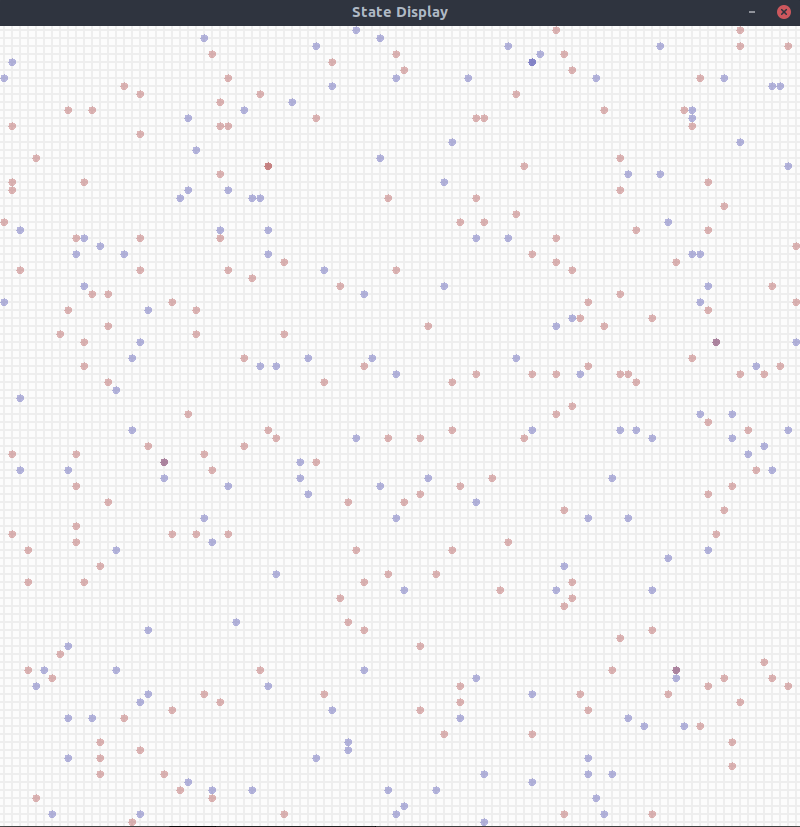
\includegraphics[scale=0.35]{images/grid.png}
\captionsetup{justification=centering}
\caption{Grid representing the city map. Each point represents a pickup or drop off location.}
\label{grid}
\end{figure}

For each person in the set N we will have two points of the grid:

\begin{enumerate}
  \item Point $i$: Is the origin place for each user (Home).
  \item Point $j$: Is the destination place for each user (Work). 
\end{enumerate}

The calculation of the distance between two points of the city will be made using the Manhattan function: 

$$ d(i,j) = \mid i_x - j_x\mid+ \mid i_y - j_y\mid $$
where $i_x$ and $i_y$ are the coordinates $x$ and $y$ of the $i$ point in the grid. 

Each user of the service will leave home at 7am and has to arrive work before 8am and the highest speed in the city is $30\ km/h$.
With the previous restrictions, supposing that the speed always is $30\ km/h$ and supposing that picking up and dropping off people don't have penalization time, we can do the following reasoning.

$$ dist = speed * time = 30\ km/h * 1\ h = 30 km $$
So each driver at most can drive $30\ km$.

Everyone who drives a car will be the first to leave and the last ones to arrive.

Also, in each car can be at most three people at the same time (including the driver).

We will have two criteria in order to evaluate the quality of the solution:
\begin{itemize}
  \item Minimize the distance traveled for each driver.
  \item Minimize the distance traveled for each driver and minimize the number of drivers.
\end{itemize} 
 
\section{Representation of a problem state}
We need a way to represent a state of the problem that is small in memory, but at the same time easy and quick to work with.
We want to avoid storing unuseful or redundant information, unless we clearly think that that information will help us reduce the computation time. Also, we want to be able to represent all the possible states that could exist.

Our states contain the following information:

\begin{itemize}
	\item Which users act as drivers and are providing their cars.
	\item For each driver, which users (passengers) the driver needs to pick up and drop off, if any.
	\item The order in which a driver needs to pick up and drop off its assigned passengers.
	\item The total distance each car will be travelling for its route.
\end{itemize}

All users (both drivers and non drivers) have a unique identifying number (id), taken from the position they occupy in the users list.
So in our state representation we will be using these identifiers to refer to users.

We consider that the order in which a car picks up and drops its passengers is important. For example, if driver A is assigned passengers B and C, there are four possible routes after leaving its home, and before arriving at work:

\begin{itemize}
	\item Pick up B, pick up C, drop off B, drop off C.
	\item Pick up B, drop off B, pick up C, drop off C.
    \item Pick up C, pick up B, drop off C, drop off B.
    \item Pick up C, drop off C, pick up B, drop off B.
\end{itemize}

These four options will result in different routes with potentially different total distances.

For this reason, we decided to use an ordered list to describe which passengers a driver needs to take care of, and the specific route they will use in the process.

Specifically, for each driver, we use a Java ArrayList listing all the sequential pick ups and drop offs of users that have been assigned, describing unambiguosuly a route that the driver needs to follow.

Continuing with the previous example, if driver A has id 1, and passengers B and C have ids 2 and 3 respectively, the first route proposed before will be stored like this: $$[1, 2, 3, 2, 3, 1]$$

In a different state, maybe the second proposed route is used, in that case the list would look like this: $$[1, 2, 2, 3, 3, 1]$$

Note how each id in the list always needs to appear twice, implicitly the first time it appears indicates that that user is being picked up, and the second one indicates that the user is being droped off.

Also note how the driver of the car is always the first and last element of the list, to represent the fact that the route must start at the driver's home, and end at the driver's workplace.

Because a state can describe the presence of many different cars (each one with its own driver, passengers, and route) we use an ArrayList to contain all the cars lists described before. Thus, we end up with the following data structure:

\begin{lstlisting}lstinlinelstinline
ArrayList<ArrayList<Integer>> assignments;
\end{lstlisting}

Apart from this, we also decided to use an extra data structure that contains the total route distances for each car:

\begin{lstlisting}
ArrayList<Integer> distances;
\end{lstlisting}

Where the distance for the route in \raggedright\lstinline{assignments[i]} is stotred in \raggedright\lstinline{distances[i]}.

Although not strictly necessary (because this could be computed at runtime from other existing data), this \lstinline{distances} variable will help us calculate the heuristic value of the state quicker. We just make sure to update these values any time \lstinline{assignments} is changed.


\begin{figure}[H]
\captionsetup{justification=centering}
\centering
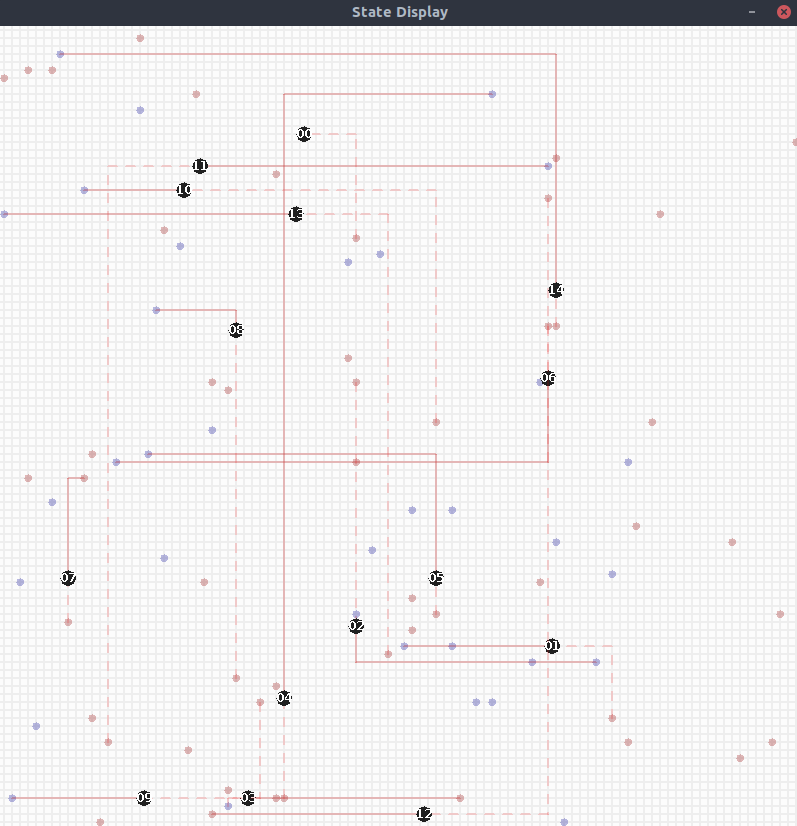
\includegraphics[scale=0.35]{images/carsMoving.png}
\caption{Visual respresentation of a moment of the state where the car is picking up and droping off people.}
\label{grid}
\end{figure}

\section{Generating an initial solution}
We have to make a representation fo the initial state, which at the same time is a solution state. We have implemented four different ways to generate our initial state: (The following examples will be done with 4 people Pi (excluding drivers), 2 drivers Di and each List will represent a car. The first time that a person appears in a List is when it is picked up and the second one when it is dropped out)
\begin{enumerate}
\item Assigning in a balanced way all the people that are not drivers in all cars, each car has the same number of people. Each person that isn't a driver will be picked up and droped of consecutively.
$$[D1,P1,P1,P2,P2,D1]$$
$$[D2,P3,P3,P4,P4,D2]$$
\item Assigning in a balanced way all the people that are not drivers in all cars, each car has the same number of people. Each car will pick up all the people and then will drop thme in the inverse order.
$$[D1,P1,P2,P2,P1,D1]$$
$$[D2,P3,P4,P4,P3,D2]$$
If the number of people that are not a driver is more than 2 times the number of drivers, this initial state will not be a goal state because the number of people in the same time in a car will be greater than 3.
\item Taking all the people that are not drivers inside the first car's list. Each person that isn't a driver will be picked up and droped of consecutively.
$$[D1,P1,P1,P2,P2,P3,P3,P4,P4,D1]$$
$$[D2,D2]$$
Because of the fact that everybody that is not a driver is in the first car it is very probable that the distance traveled by the first car will be more than $30\ Km$ and that initial state won't be a goal state.
\item Taking all the people that are not drivers inside the first car's list. Each car will pick up all the people and then will drop thme in the inverse order.
$$[D1,P1,P2,P3,P4,P4,P3,P2,P1,D1]$$
$$[D2,D2]$$
If the number of people that are not a driver is more than 2, this initial state will not be a goal state because the number of people in the first car will be greater than 3. Although, because of the fact that everybody that is not a driver is in the first car it is very probable that the distance traveled by the first car will be more than $30\ Km$ and also, that initial state won't be a goal state.
\end{enumerate} 

\section{Analysis of our operators}

Once we have defined the structure we will work with, we have to decide which operators will modify our structure to move from one  state to another. To do this, we must take into account several factors, so that when executing our algorithm, the best possible solution is found in a fairly reasonable execution time. 
\\
Our operators indicate all the possible paths that can be taken given any state. Then we will use all these possibilities with the objective that this becomes a state with some favorable characteristics. This is called a branch factor and it changes the way it is applied depending on which algorithm we are using. In the \textbf{Hill Climbing}, we generate all the successors and the heuristic decides if it is good enough to stay with him, in the \textbf{Simulated Annealing} we generate a successor status in a random way and the heuristic decides if it is good enough to stay with him. 
\\
\medskip

It is really important to cover all the space of solutions with our operators because if we are not doing it, there may exist solutions that will be lost, which could prevent us from reaching an optimal solution. Also we be cautious about creating repeated solutions because our execution time would be affected. 
\\

At the beginning of everything we made a brainstorming session with all the operators we could think of, which we believed that could be useful and serve for something: swap the order of the people inside a car, swap outside people between cars, deleting cars, moving a person into another car, etc...

Finally we decided to implement these 3 operators, which we think they would reach to all the possible solutions:

\begin{enumerate}
\item \textbf{Move}: this operator lets us move any person that is not a driver from the car $i$ to another car $j$, in a pickup place $k$ and a drop off place $l$.  
\item \textbf{Swap inside}: this operator lets us swap the order of the people inside a car $i$.
\item \textbf{Delete car}: this operator lets us delete a car whenever the car is only occuped by the driver. When the deletion is made the driver is inserted into another car. 
\end{enumerate}



\section{Generating successor states}
The way we generate all the successor states really varies depending on the algorithm:
\begin{itemize}
\item \textbf{Hill Climbing}: we create a list with all the possible states that can be found from the given one. To do it, we create all the possible states that can be created using our operators, previously explained in section above. Then Hill Climbing will use our Heuristic Function to choose the best successor.
\item \textbf{Simulated Annealing}: we return a random state that is a succesor of the given one. To do it, we choose a random operator with random values. Then we use it in order to change the initial state.  
\end{itemize}

\section{Goal State}

In our experiment we will have two conditions in order to determinate if a state is a goal state:

\begin{enumerate}
  \item The distance of each car has to be at most $30\ Km$. In order to do this, we have a variable in state objects with his distance, and we obtain it directly.
  \item At the same time can be at most three people in each car. In this case, we have a function in the object state, which computes the exceed of simultaneous people in a car. The penalization will be worst as higher is the value.
\end{enumerate}

\section{Heuristics Function} \label{heuristics}
Once the representation of the solution state has been defined, the generation of the initial solution state and the operators on which we are going to work, we proceed into analysing the heuristic function. 

In order to solve the two solution criteria given in the statement, we must perform two different heuristics, because the final result that must be returned has different priorities. The heuristic function that will solve the first criterion will be called Heuristic Function 1, and the one that resolves the second, Heuristic Function 2. 

\subsection{Heuristic Function 1}

The criterion that this function must follow is quite simple, the objective is to minimize the sum of all the distances that each car has to do and minimize the maximum number of people at the same time in each car.

To follow this criterion, we will compute the heuristic value of each state following this criteria.

\begin{enumerate}
  \item Compute the sum of distances that each car exceed. Each state has an ArrayList with the distance that every car drives, so iterating this array we will obtain the distance of all cars. We will only catch the ones that exceeds the limit of $30\ Km$, penalizing this situations.
  \item Compute the sum of people that each car carries in a certain moment of the travel. Here for each car with the list of pick up and drop out people we can find the maxim number of people in a certain moment. The values that exceeds the maximum of 3 people for car at the same time, are used in order to penalize this situations.
\end{enumerate}

\subsection{Heuristic Function 2}

For the second heuristic we have added another criterion in order to minimize also the number of cars that are driving. 

\begin{enumerate}
  \setcounter{enumi}{2}
  \item Get the number of cars in each state. Adding the sum of previus criterias a ponderate value of the number of cars, we obtain this second heuristic.
\end{enumerate}

\section{Experiments}

\subsection{Experiment 1}
In this experiment we will decide which is the best operator of the different ones we have created using the \textit{Heuristic Function 1}. 
\\
\medskip 

This experiment is going to be made using \textbf{200 people }($N$), and \textbf{100 drivers }($M$), using \textbf{10 random seeds} and executing only the \textbf{Hill Climbing algorithm}. In order to perform it, firstly, we will have to generate an initial solution. From all the possible initial solution generators that we have implemented, we have chosen the third one, since we believe that is the one that gives us the best results (this fact is going to be proven in the \textit{Experiment 2}). 

As we mentioned in the previous section \textit{Analysis of our operators}, we have three different operators. In order to try out which set of operators is the best one, we have automatized a process where all different operators are applied to the scenery using different seeds to see which one gives us better results and better time. 
\\
Our \textbf{hypothesis} is that a combination of all of them will gives us the best results because using all of them will let Hill Climbing find the path to the global maximum. 

\begin{figure}[H]
\centering
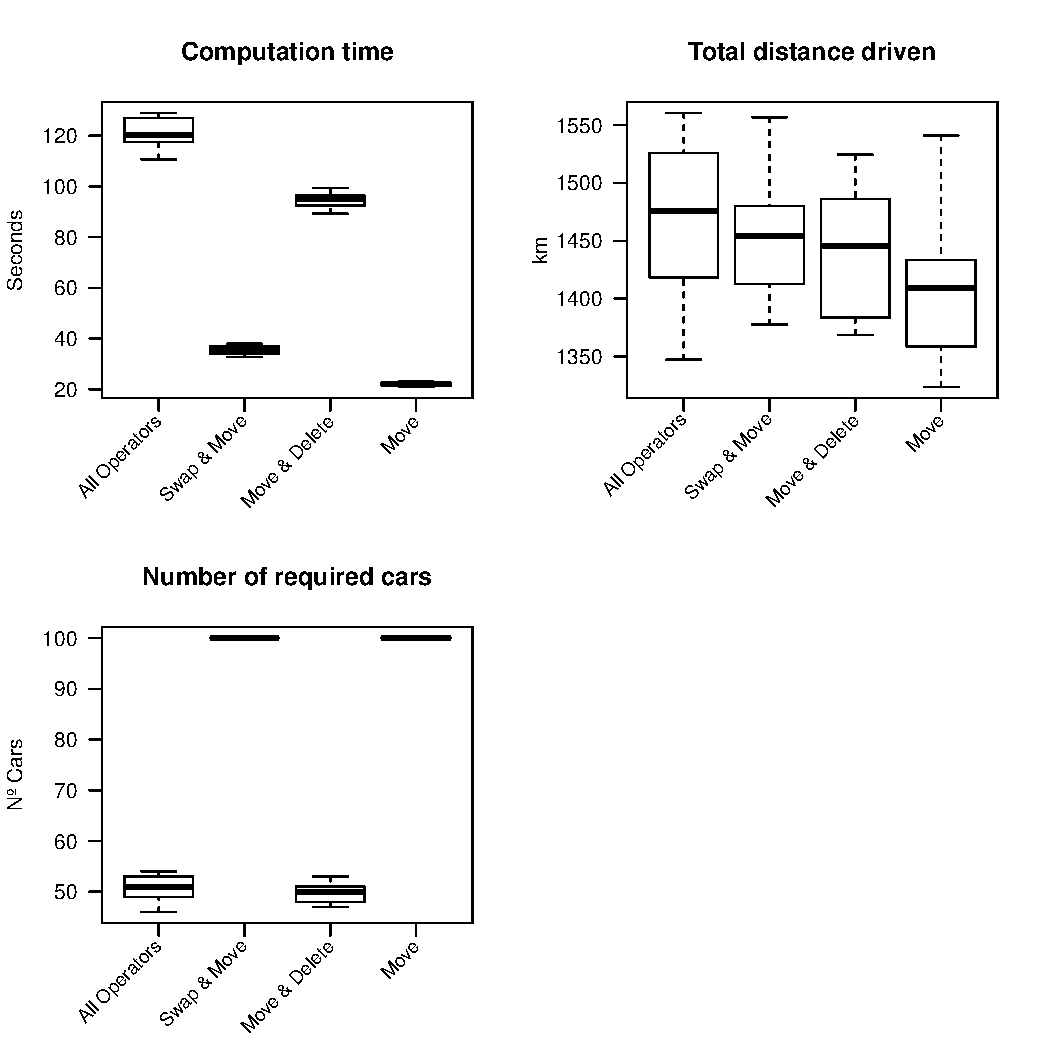
\includegraphics[width=\textwidth,height=\textheight, keepaspectratio]{Results/data_1.pdf}
\caption{Plots with different parameters measured for each operator }
\label{operators}
\end{figure}
\vspace{1cm}

Finally after getting \textbf{the results}, clearly seen in the figure \ref{operators}, we can see that our hypothesis about the operators was wrong. Let's analyse our results for each parameter: 
\\
\smallskip

If we take a look into the Computation time, we can see that the worst solution is obviously the one using all the operators since it creates several more successors. So in terms of time we conclude that it is the worst solution. However, to get a correct idea about the best operators we should look before into the solutions we got. 
\\
\smallskip

The total distance results are pretty similar in all the methods. The best one is \textbf{Move}, because it is not able to delete the number of cars created in the initial solution so it can only minimize the distance.  
\\
\smallskip

When we analyse the number of required cars we discover that the best solutions are the ones that uses \textbf{All Operators} and \textbf{Move} and \textbf{Delete}. The difference here between solutions is really huge because the other operators are not  able to delete cars. 


It is interesting to observe that we did not tried some operators alone like \textit{swap inside} or combination of them like \textit{swap inside} and \textit{delete} . The main reason for the decision is that the operator \textit{swap inside} alone would never give us a solution state since our first state includes a car with too much people in a single car(for more information about the initial solution please check \textit{Generating an initial solution, version 3}). 
\\
\smallskip

\paragraph{Conclusion}\mbox{}\\
The best set of operators for \textbf{Hill Climbing} is \textbf{Move} and \textbf{Delete}. Taking in account that the time taken is pretty acceptable, it is the best solution in the number or required cars and it gets good results in the total distance driven.

\subsection{Experiment 2}
We did this experiment in order to know which was the most suitable way to generate our initial solution. In this experiment we will use the best set of operators available found in the previous experiment.

We will use \textbf{the same scenery that was used in the first experiment} ($N=200$ and $M=100$ and $10$ executions using random seeds).  In order to try all the different initial solution generators we have created a process where the same scenery is applied to different initial solution methods to see which one gives us better results and better time. 

Our \textbf{hypothesis} is that the best solution will be the first or the second one, those solutions assign in a balanced way all the people that are not drivers in all cars (if you want to know more about it please check the section \textit{Generating an initial solution}). Our hypothesis is based on the belief that starts already in an stable place, pretty close to the optimal solution; so it will not last a lot of time finding the best solution. 

\begin{figure}[H]
\captionsetup{justification=centering}
\centering
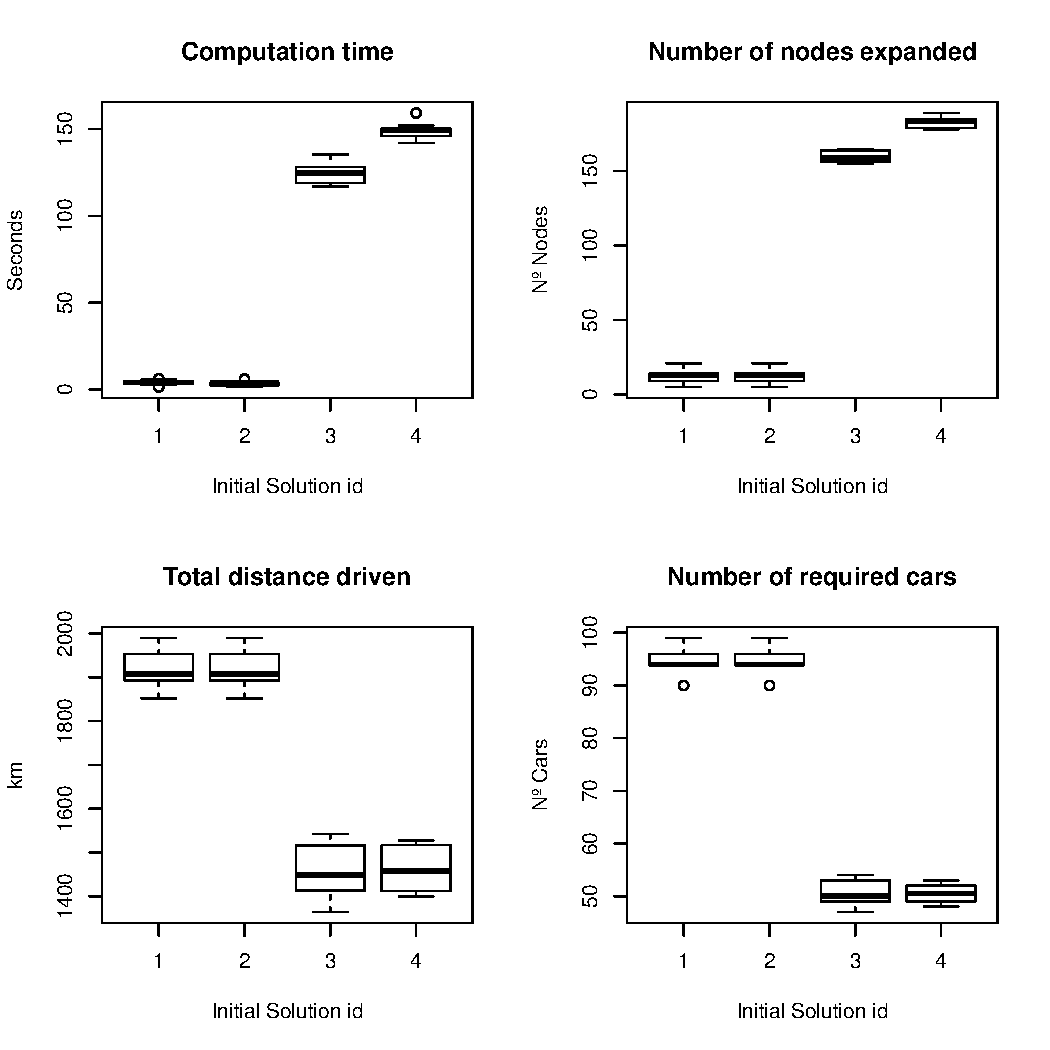
\includegraphics[width=\textwidth,height=\textheight, keepaspectratio]{Results/data_2.pdf}
\caption{Plots with different parameters measured for each intial solution.}
\label{operators}
\end{figure}

\paragraph{Observations}\mbox{}\\
\begin{enumerate}
\item Initial solutions nº 1 and nº 2 expand a very small number of nodes, as a result, they take very little computation time,
but also provide very poor final solutions: the number of cars is barely reduced, and the total distance driven is relatively high.

\item Initial solutions nº 3 and nº 4 expand a large number of nodes before stopping, resulting in higher computation time,
but end up providing a much more optimal final solution, with almost half the number of cars as before, and significantly reducing the total distance driven.

\item Initial solution nº 3 requires less computation time than solution nº4, while still providing similar (if not better) final results.

\end{enumerate}

\paragraph{Conclusion}\mbox{}\\
Initial solution nº 3 seems to be the best initial solution out of the 4 we proposed.
From now on, we will be only using initial solution nº 3 for our experiments.

\subsection{Experiment 3}

A really important part about this project is to be able to determine the parameters that are going to be used for the \textbf{Simulated Annealing algorithm}, so that its results are the best possible, that is, the minimum number of cars driving the shortest amount of distance and everybody getting to their workplace in a reasonable execution time. 
\\
\medskip

The algorithm works with 4 parameters:
\begin{enumerate}
\item \textbf{Steps}: The total number of iterations that the algorithm will perform. 
\item \textbf{Number of iterations for each temperature change}: Whenever there is a temperature change, a constant number of iterations will be made in which the probability of choosing a worse successor is kept. 
\\
Each time this number of iterations is executed, the probability of choosing a worse state decreases. 
\item \textbf{k}: parameter of the state acceptance function that affects the probability of choosing a worse succesor state. We know that the higher the value of the parameter, the longer it takes for the probability of staying with a worse successor state to decrease. 

\item \textbf{$\lambda$}: Another parameter of the state acceptance function that affects the probability of choosing a worse successor. The higher the value of $\lambda$, the less it will take to decrease the probability of accepting a worse successor state. 


\end{enumerate}


Since there are several parameters, our \textbf{hypothesis} is that there must exists an exact combination of them which will allow Simulated Annealing to give us the best solutions. In order to do it, we have used \textbf{same scenery used in the previous experiments} ($N=200$ and $M=100$) but setting the seed to a fixed value (\textbf{1234}) since Simulated Annealing is already random in its core and it will change in every execution. Then we measured different parameters of each execution and created several plots in order to discuss in the best way possible its results. 

    \begin{figure}[H]
    \captionsetup{justification=centering}
    \centering
        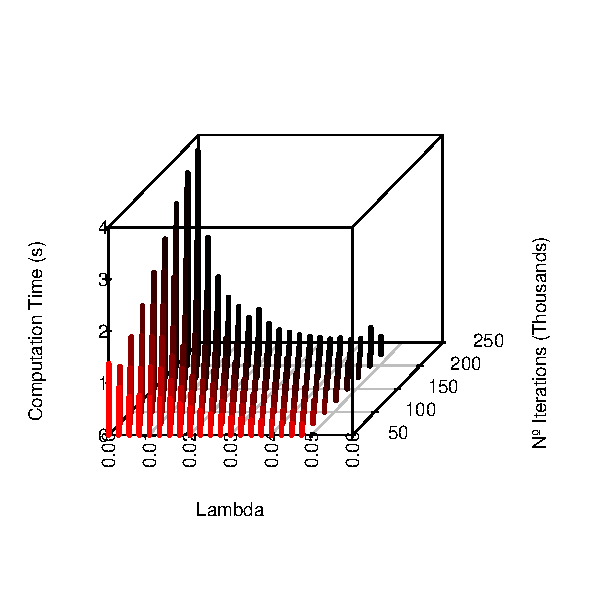
\includegraphics[scale=0.9]{Results/data_B_1.pdf}
        \caption{Time values ($s$) related to $\lambda$ and number of iterations}
        \label{fig:data2}
    \end{figure}
    
In the figure \ref{fig:data2} we can see that there is a clear relation between the time and the $\lambda$ and the total number of iterations (or so called steps). We can see that as lambda and number of iterations grows the time also grows with them.     
    
    \begin{figure}
    \captionsetup{justification=centering}
   		\centering
        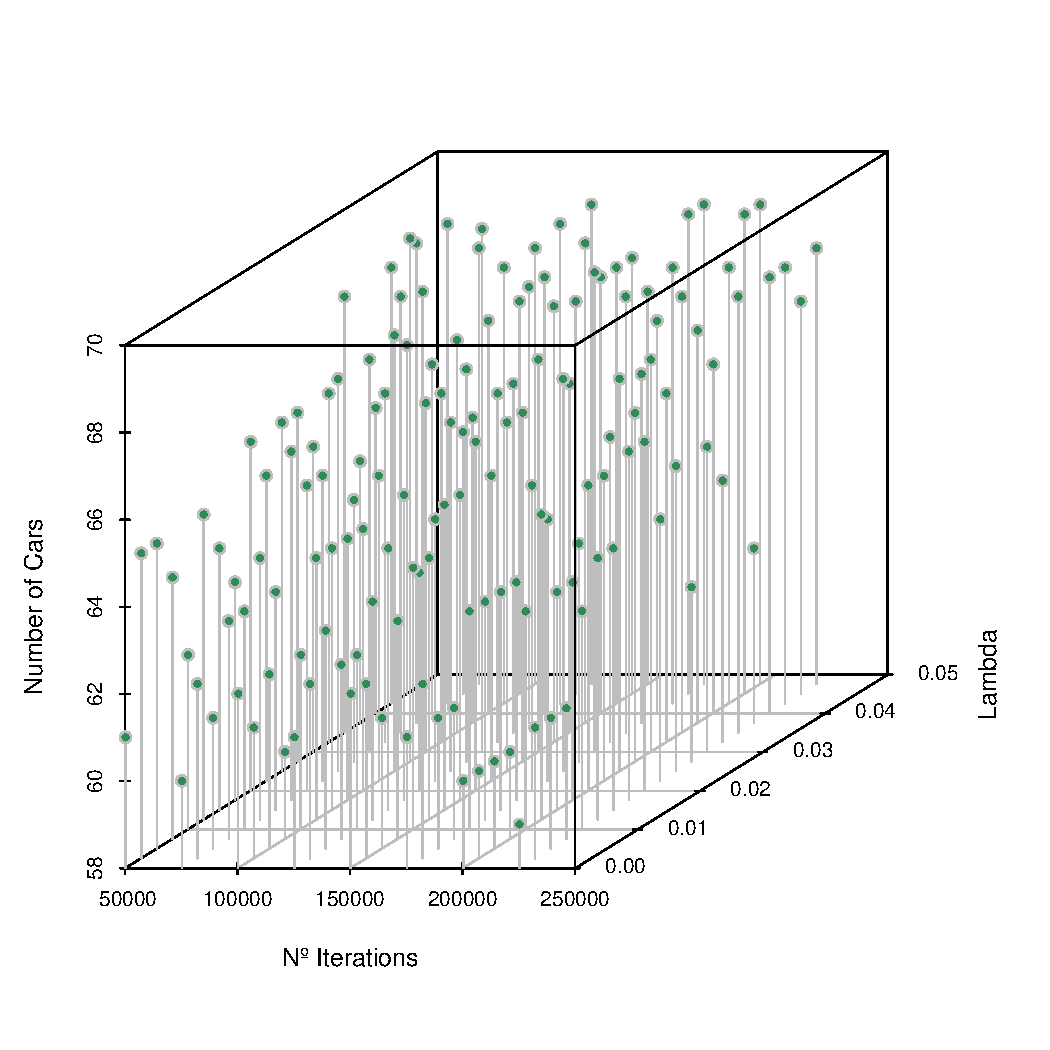
\includegraphics[scale=0.9]{Results/data_B_2.pdf}
        \caption{Number of cars of the final state related to number of iterations and $\lambda$}
        \label{fig:data3}
    \end{figure}
        
        \vspace{1cm}
In the figure \ref{fig:data3} we can see the relation between the total number of cars and the $\lambda$ and the number of iterations. In this case the relationship is not so  obvious as the previous case, a really small declining tendency is distinguished along the number of iterations, but as the lambda grows it becomes not so obvious. However if we just take a look into the $\lambda$ values we can see a higher number of cars the higher it is. So, taking in account that we want to minimize the numbers of cars, we can conclude that the best values are a small $\lambda$ and a big number of iterations. 
       
       \begin{figure}
       \captionsetup{justification=centering}
       \centering
        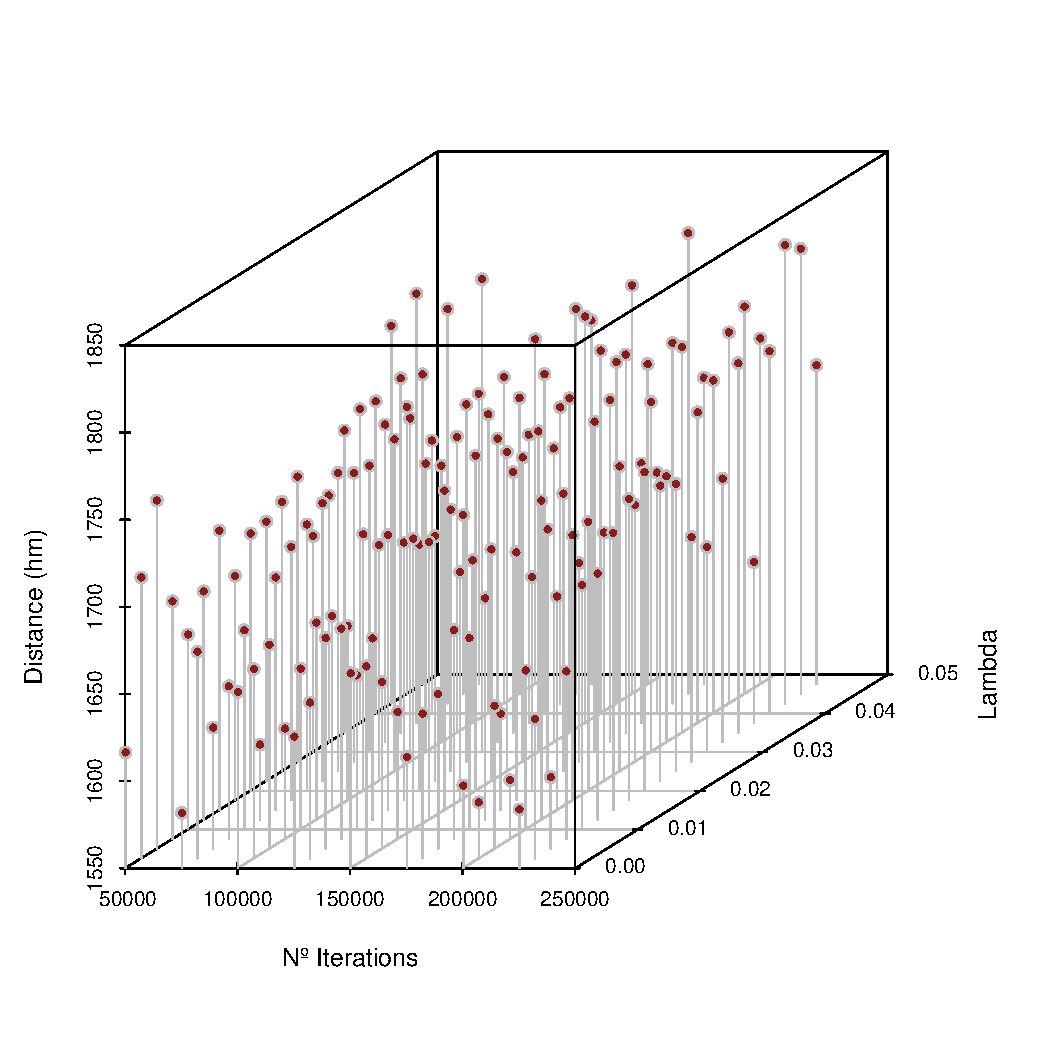
\includegraphics[scale=0.9]{Results/data_B_3.pdf}
        \caption{Total distance of the final state ($km$) related to the number of iterartions and $\lambda$.}
        \label{fig:data4}
    \end{figure}
      \vspace{1cm}
In the figure \ref{fig:data4} we can see the relation between the total distance and the $\lambda$ and the number of iterations. In this case we can conclude that the higher the lambda the higher the total distance. Moreover, it happens exactly the same with the number of iterations. This observation supports the previous analysis with the number of cars since a smaller value of cars is heavily related to a smaller value of total distance. So using this plot we can confirm the affirmation of small values for lambdas and big number of iterations as the best options. 
    
    
    \begin{figure}[H]
    \captionsetup{justification=centering}
     \centering
      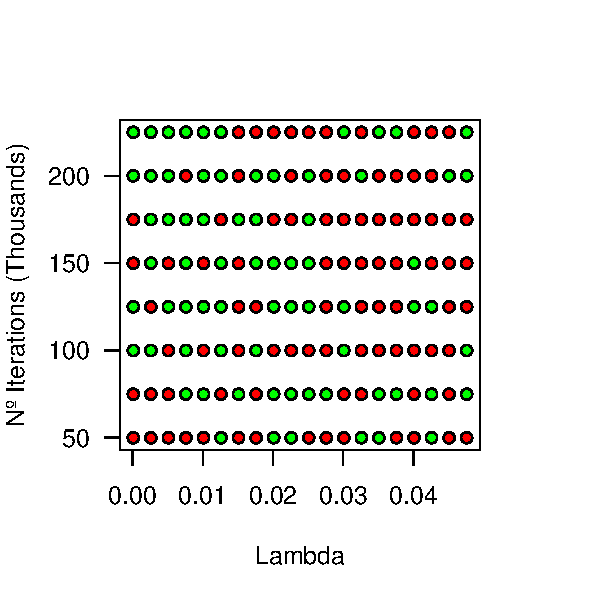
\includegraphics[scale=0.8]{Results/data_B_4.pdf}
        \caption{Distribution of the final states that were solutions depending on the number of iterations and $\lambda$}
        \label{fig:data5}
    \end{figure}
      \vspace{1cm}
Also, we wanted to finally conclude with a plot showing how usually is not to arrive to a solution state. We can see in the figure \ref{fig:data5} a plot showing if an execution arrived to a solution (green color) or not (red color). Even though we though that the $lambda$ values and the number of iterations would present a heavy relationship in the distribution, we did no obtain it. 
 \\
 \medskip
About the presence of states that are not solution: we believe that this happens mainly due to the randomness that Simulated Annealing presents and because we pushed to the limit our heuristic in order to get the best solution and sometimes we get a car that drives slightly more than the maximum allowed. 


%
%\begin{figure}
%\centering
%
%    ~ %add desired spacing between images, e. g. ~, \quad, \qquad, \hfill etc. 
%      %(or a blank line to force the subfigure onto a new line)
%    \begin{subfigure}[b]{0.3\textwidth}
%        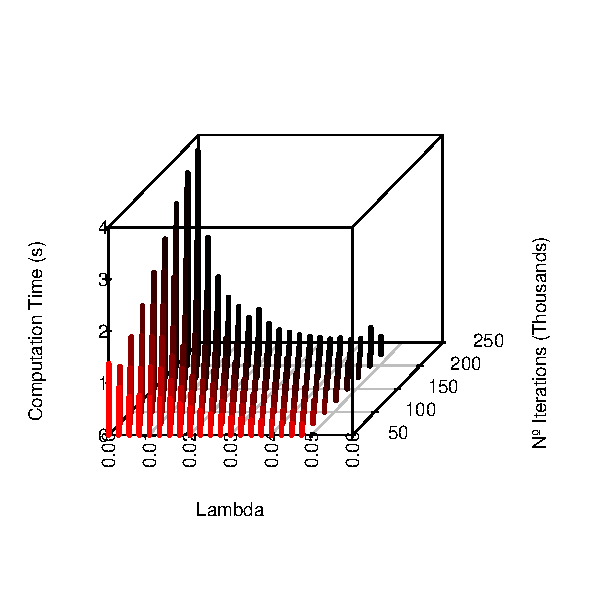
\includegraphics[width=\textwidth]{Results/data_B_1.pdf}
%        \caption{Time values ($ms$) related to lambda values and number of iterations}
%        \label{fig:data2}
%    \end{subfigure}
%    \begin{subfigure}[b]{0.3\textwidth}
%        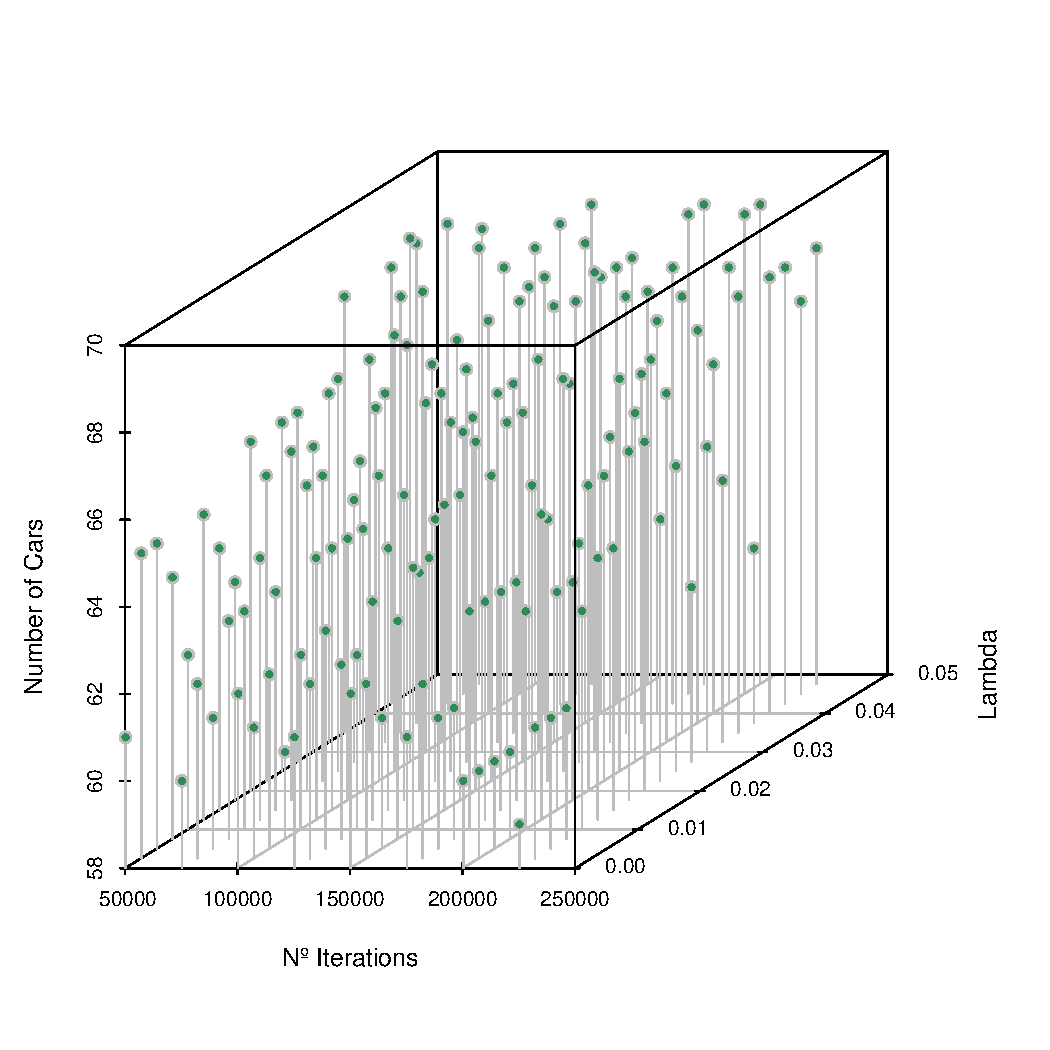
\includegraphics[width=\textwidth]{Results/data_B_2.pdf}
%        \caption{Number of cars of the final state related to number of iterations and lambda values}
%        \label{fig:data3}
%        \end{subfigure}
%            \\
%            
%       \begin{subfigure}[b]{0.3\textwidth}
%        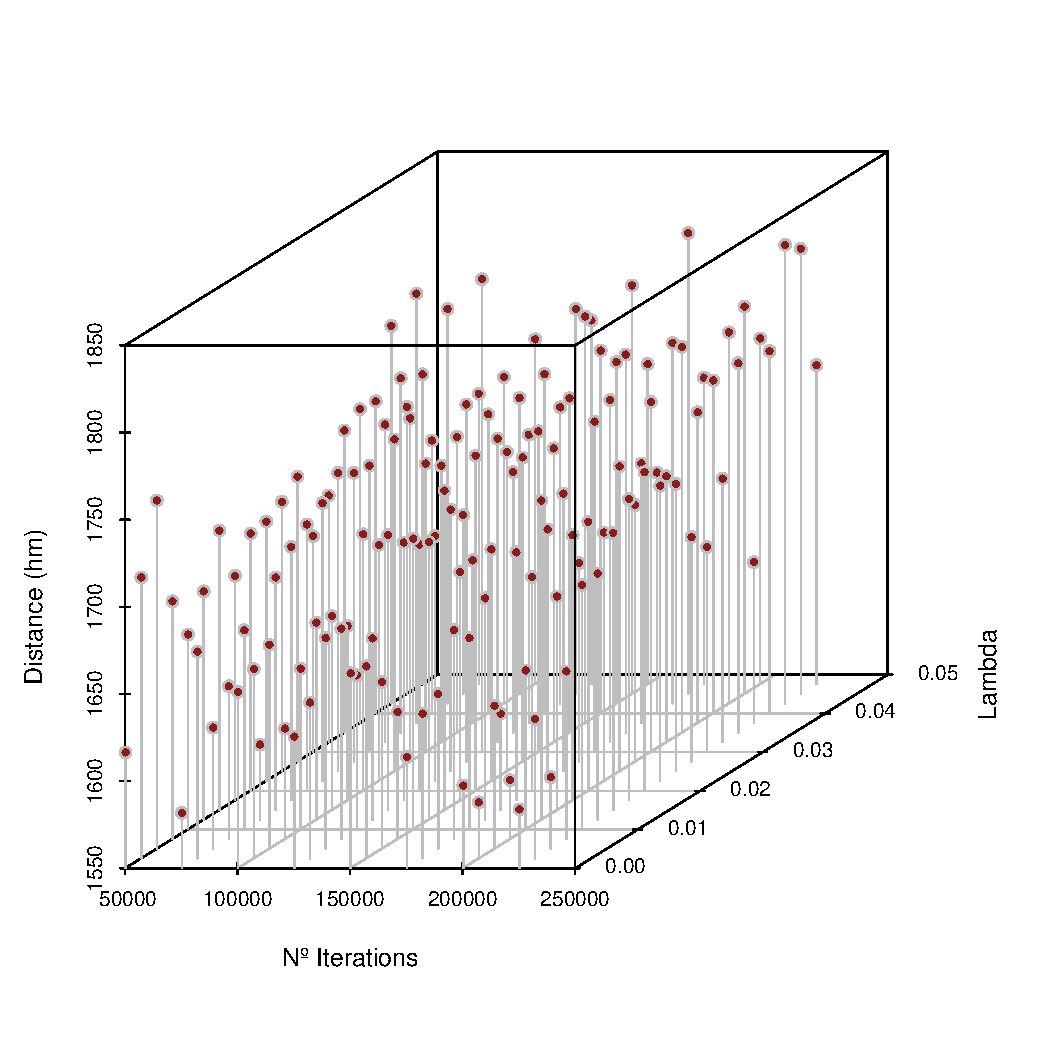
\includegraphics[width=\textwidth]{Results/data_B_3.pdf}
%        \caption{Total distance of the final state ($hm$) related to the number of iterartions and lambda values.}
%        \label{fig:data4}
%        \end{subfigure}
%     \begin{subfigure}[b]{0.3\textwidth}
%      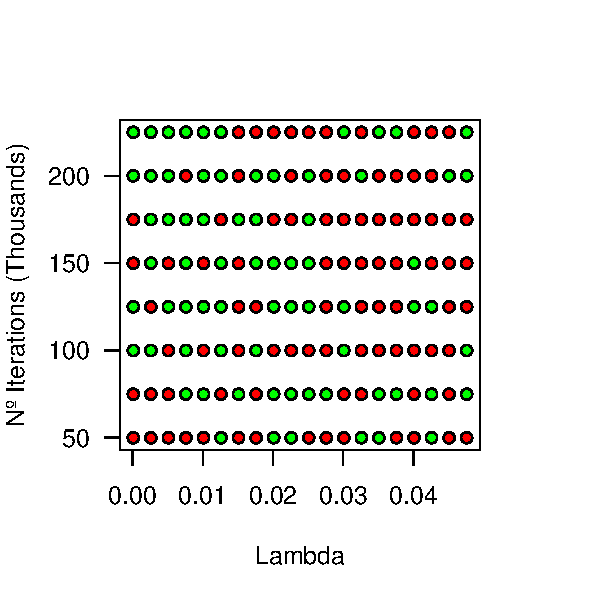
\includegraphics[width=\textwidth]{Results/data_B_4.pdf}
%        \caption{Distribution of the final states that were solutions depending on the number of iterations and lambda values}
%        \label{fig:data5}
%    \end{subfigure}
%    \caption{Plots of our experiments with Simulated Annealing parameters: Lambda and Number of total iterations (steps)}\label{fig:plotSimulated}
%\end{figure}

\paragraph{Conclusion}\mbox{}\\


\subsection{Experiment 4}
\textbf{Using the same scenery we have used in the previous experiments}($N=200$ and $M=100$) we will be studying how the execution time changes to find the solution  assuming a proportion of $\frac{M}{N}$ of $\frac{1}{2}$. The experiment will be run using the     
 \textit{Hill Climbing} algorithm and a random seed that is fixed since at each iteration we are already varying the sizes of $N$ and $M$.

We have started with $200$ users and then, each iteration, we have incremented by $1000$ the users until we have discovered a pattern. Our \textbf{hypothesis} is that the time is going to be heavily influenced by the size of $N$. Actually we think that they are going to be directly proportional. 

\begin{figure}[H]
\centering
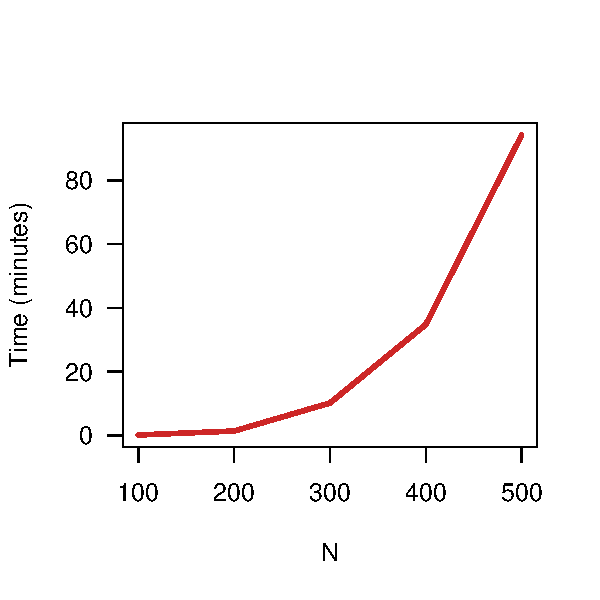
\includegraphics[scale=0.8]{Results/data_4_1.pdf}
\caption{Computation time measured for different numbers of people (N), and drivers (N/2)}
\label{timedifferentN}
\end{figure}
\vspace{1cm}

As we can see in the previous figure \ref{timedifferentN}, there is a clear pattern: as the size of N grows, the time augments really fast (exponentially). We believe that the main reason for this behavior is because the number of nodes that are going to be created for each iteration is expanded exponentially as the $N$ grows. If you want to see more about why the number of successors that are created please check the \textit{Generating successor states} and \textit{Analysis of our operators}

\paragraph{Conclusion}\mbox{}\\

\subsection{Experiment 5}
In the assignment we had two main objectives: minimize the distance driven and minimize the cars that are needed. To make it we have implemented two heuristic functions. 

DUring some experiments we find that the best way in order to minimize the distance is minimizing also the cars. So we finally have chosen to apply all of the experiments with the second heuristic.

In order to study how the heuristic functions work, we will observe the total distance driven, the execution time and the total number of cars. We will use the \textit{Hill Climbing} algorithm.

As it is explained in the section \ref{heuristics} we have three diferent types of penalties. To do this experiment we will force the value of the max number of people in the same time and we will be varying the other two.

%MIRAR ENUNCIAT QUE DIU QUE En este caso tendréis que buscar como se han de ponderar los criterios de la segunda heurística. 

\begin{figure}[H]
  \captionsetup{justification=centering}
   \centering 
    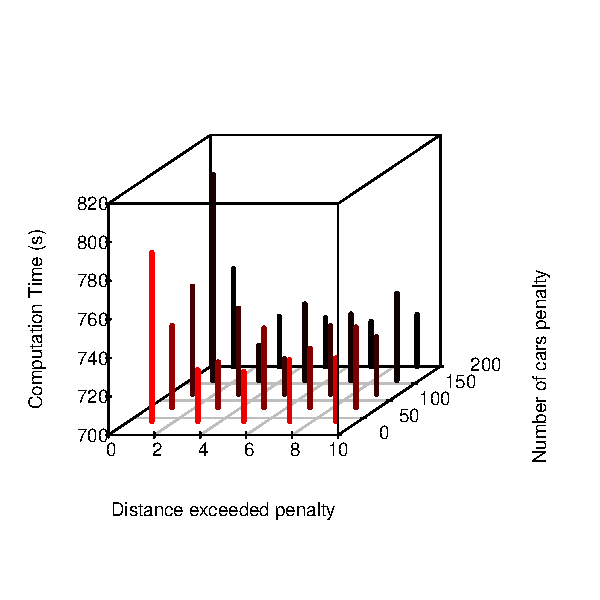
\includegraphics[scale=0.8]{Results/data_5_1.pdf}
      \caption{Computation time measured for different penalties in the number of cars and distances using Hill Climbing}
      \label{fig:data_5_1}
  \end{figure}
    \vspace{1cm}

In the Figure \ref{fig:data_5_1} we can see that the execution time is bigger when the distance exceed penalty is small, when this value increases the time turns constant.

\begin{figure}[H]
  \captionsetup{justification=centering}
   \centering
    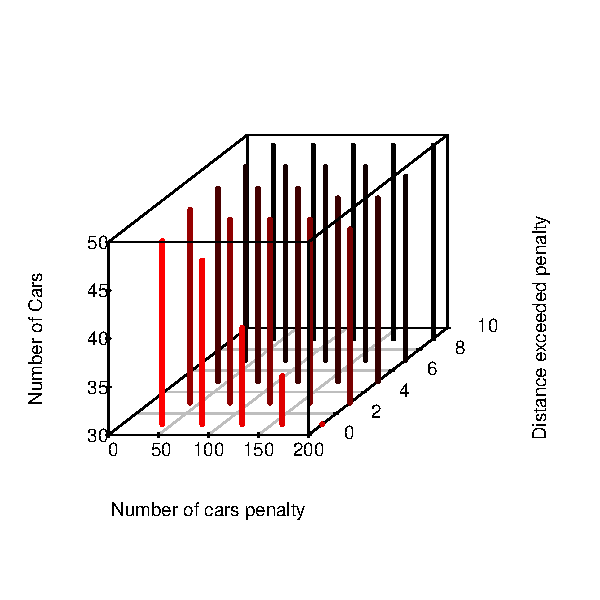
\includegraphics[scale=0.8]{Results/data_5_2.pdf}
      \caption{Number of cars measured for different penalties in the number of cars and distances using Hill Climbing}
      \label{fig:data_5_2}
  \end{figure}
    \vspace{1cm}

In the Figure \ref{fig:data_5_2} the important changes are seen when the distance exceed penalty is lower and when the cars penalty is bigger. 

\begin{figure}[H]
  \captionsetup{justification=centering}
   \centering
    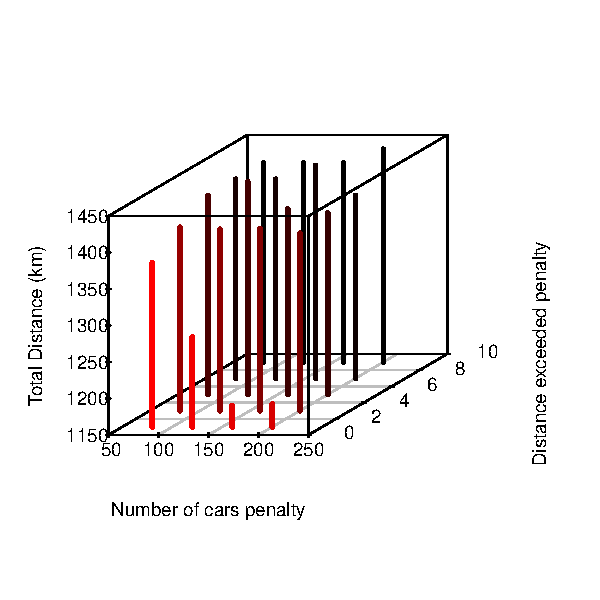
\includegraphics[scale=0.8]{Results/data_5_3.pdf}
      \caption{Total distance measured for different penalties in the number of cars and distances using Hill Climbing}
      \label{fig:data_5_3}
  \end{figure}
    \vspace{1cm}

In the Figure \ref{fig:data_5_3} we can see a very similar comparing with the Figure \ref{fig:data_5_2}. When the number of cars penalty increases and when the distance exceeds is being smaller we have better results.

\begin{figure}[H]
  \captionsetup{justification=centering}
   \centering
    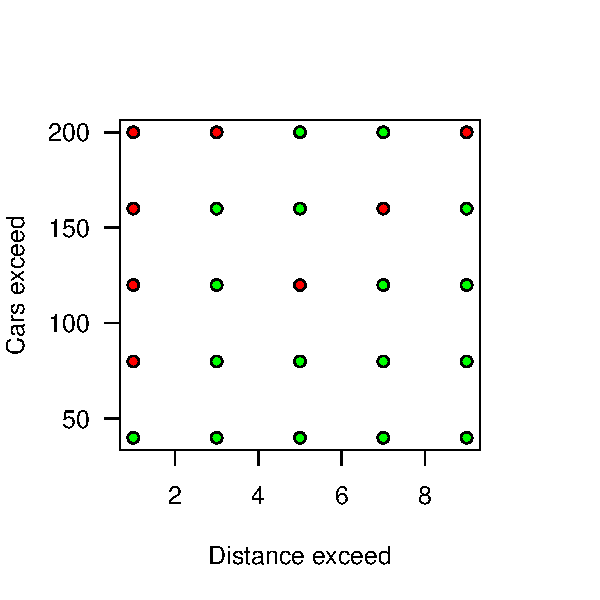
\includegraphics[scale=0.8]{Results/data_5_4.pdf}
      \caption{Correctness for different penalties in the number of cars and distances using Hill Climbing}
      \label{fig:data_5_4}
  \end{figure}
    \vspace{1cm}

The las Figure of this experiment (Figure \ref{fig:data_5_4}) shows the correctness of each penalty.
    
\paragraph{Conclusion}\mbox{}\\

To conclude we will choose a penalty both ponderations. Watching the results we can abstract that a lower value of the number of cars penalty and with a value in the middle of the possible distance exceed penalty it might be the best one.
Finally we have chosen tha value of 5 in the distance and 80 for the car penalty, because it is a correct solution for this seed and because the complexity and the solutions seems better.

\subsection{Experiment 6}
Using the same scenarios used before, we repeated the executions with the Simulated Annealing algorithm with the chosen heuristic.

\begin{figure}[H]
  \captionsetup{justification=centering}
   \centering
    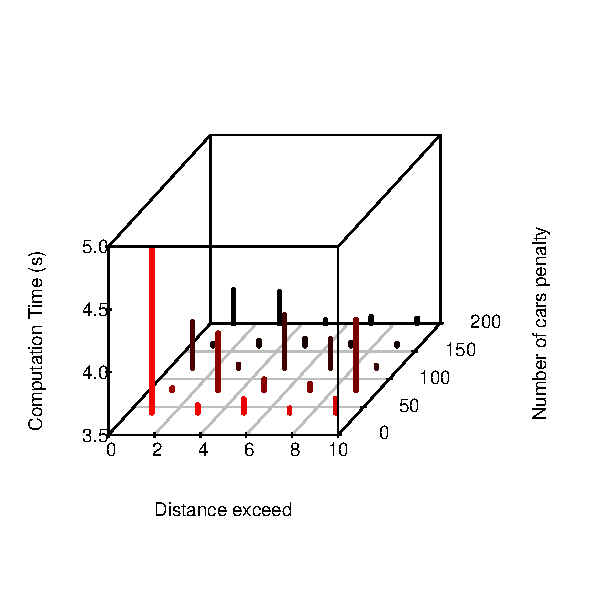
\includegraphics[scale=0.8]{Results/data_6_1.pdf}
      \caption{Computation time measured for different penalties in the number of cars and distances using Simulated Annealing}
      \label{fig:data_6_1}
  \end{figure}
    \vspace{1cm}

\begin{figure}[H]
  \captionsetup{justification=centering}
   \centering
    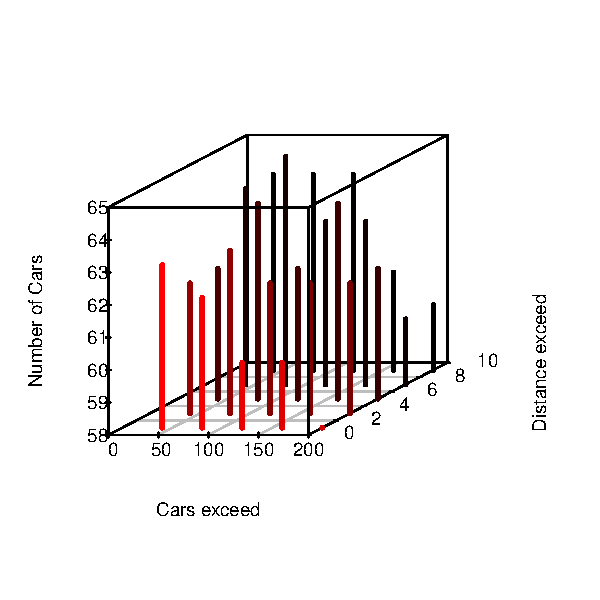
\includegraphics[scale=0.8]{Results/data_6_2.pdf}
      \caption{Number of cars measured for different penalties in the number of cars and distances using Simulated Annealing}
      \label{fig:data_6_2}
  \end{figure}
    \vspace{1cm}

\begin{figure}[H]
  \captionsetup{justification=centering}
   \centering
    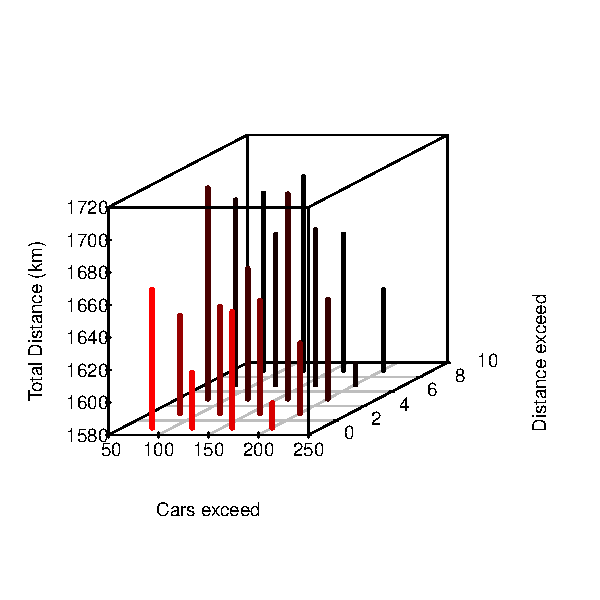
\includegraphics[scale=0.8]{Results/data_6_3.pdf}
      \caption{Total distance measured for different penalties in the number of cars and distances using Simulated Annealing}
      \label{fig:data_6_3}
  \end{figure}
    \vspace{1cm}

\begin{figure}[H]
  \captionsetup{justification=centering}
   \centering
    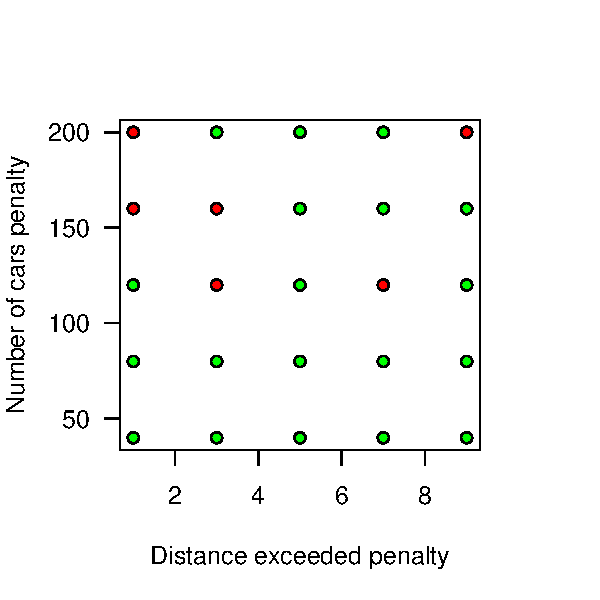
\includegraphics[scale=0.8]{Results/data_6_4.pdf}
      \caption{Correctness for different penalties in the number of cars and distances using Simulated Annealing}
      \label{fig:data_6_4}
  \end{figure}
    \vspace{1cm}
    
\paragraph{Conclusion}\mbox{}\\

\subsection{Experiment 7}
Through all the previous experiments, we have been using the same proportion of drivers($M$) towards people($M$): $N/2$. For this experiment we will be testing another proportions less conservatives. Using a smaller value of drivers will make the algorithm start in a closer spot to the solution.

In order to discover the best proportion for each size we will experiment with different values. We have used the heuristic function and algorithm that gave us the best results which are BLABLABLA as we clearly showed in the previous experiments. 

\paragraph{Conclusion}\mbox{}\\

\subsection{Especial Experiment}

At this point we have degined the best initial state, its operators, the heuristic algorithm and Hill Climbing and Simulated Annealing with the most appropiate parameters, so we can proceed to compare algorithms. 


\subsubsection{Hill Climbing}

The experiment was made configuring our environment with 200 people, 100 drivers and seed 1234.
\\

We would like to add that these results are a valid solution because no car drives more than 30 km and there is not any moment where a car carries more than 2 people. 
\\

\begin{table}[h]
\centering
\begin{tabular}{|l|l|l|l|}
\hline \textbf{Time} &
 \textbf{Nodes expanded} & \textbf{Cars} & \textbf{Distance}\\  \hline
6054 ms &  17 & 92 & 1834.3 km \\ \hline
\end{tabular}
\caption{Results of our experiments with Hill Climbing}
\label{Results}
\end{table}

\subsubsection{Simulated annealing}
The experiment was made configuring our environment with 200 people, 100 drivers and seed 1234.
\\ 


\begin{table}[H]
\centering
\begin{tabular}{|l|l|l|l|l|l|}
\hline & \textbf{Time}  & \textbf{Cars} & \textbf{Distance} & \textbf{Solution}\\  \hline
 \#1 & 2596 ms  & 62 & 1671.3 km & Yes \\ \hline
 \#2 & 1218 ms & 64 & 1678.2 km & Yes \\ \hline
  \#3 & 1044 ms & 67 & 1753.3 km & Yes \\ \hline
 \#4 & 1088 ms & 65 & 1734.8 km & Yes \\ \hline
 \#5 & 1058 ms & 63 & 1731.1 km & No \\ \hline
 \#6 & 1131 ms & 65 & 1685.2 km & Yes \\ \hline
 \#7 & 1029 ms & 65 & 1720.5 km & Yes \\ \hline
 \#8 & 1067 ms & 66 & 1777.1 km & Yes \\ \hline
 \#9 & 1088 ms & 64 & 1657.6 km & Yes\\ \hline
 \#10 & 2596 ms & 65 & 1688.5 km & Yes \\ \hline

\end{tabular}
\caption{Results of our experiments with Simulated Annealing}
\label{Results2}
\end{table}

The mean time of our executions using Simulated Annealing is 1709.76 ms. 

\section{Conclusion}


\end {document}